\chapter{Otimizacao}
\label{cap:otimizacao}
  O grmonty é um programa escrito em C que se utiliza fortemente da biblioteca OpenMP.
  Este trabalho é uma otimização de seu código, basedo principalmente em exportar
  o código para CUDA, mas para isso se faz necessário analizar a estrutura e
  funcionamento do programa, para assim encontrar pontos onde sua performance
  pode ser acrescida, usando principalmente a técnica de paralelização na GPGPU.
  Neste capítulo nos dedicamos a explanar a arquitetura na qual o grmonty opera
  e descrever pontos que poderiam ser otimizados e como poderiam, além de mostrar
  modificações necessárias para seu funcionamento na GPGPU.

\section{Arquitetura do Programa}
  ``Fazendo o design do grmonty nossa filosofia foi de maximizar a transparência
  física e minimizar o tamanho do código, ocasionalmente ao custo de redução de
  performance'' \citep{Dolence:09} (tradução nossa). Uma escolha técnica foi feita
  ao se desenvolver o grmonty, um enfoque maior na legibilidade de suas fórmulas
  físicas em detrimento da performance, uma escolha condizente com um
  código que se procura uma manutenção e estudo mais amigável, convidativa e simples.

  Um exemplo dessa prática é ao computar um percurso por uma geodésica, tarefa
  computacionalmente dispendiosa. É amplamente reconhecido \citep{ynogkm:13} que
  um esquema que depende da integrabilidade das geodésicas em um vácuo de Kerr é
  mais eficiente que integrar diretamente a equação da geodésica, porém essa segunda
  opção foi a escolhida pois é mais simples e mais curta \citep{Dolence:09}.

  Todo o código do grmonty é escrito em C, tal escolha pode ter sido feita pois
  a linguagem é extremamente veloz e possui bibliotecas muito focadas em performance, além de permitir um controle mais fino da memória e das
  operações sendo executadas. Graças a essa característica a decisão de portar o
  código para CUDA é mais fácil pois CUDA pode ser visto como uma extensão de C.

  O código do grmonty opera da forma mostrada na figura \ref{fig:grmontyGraph} seguindo o seguinte fluxo: primeiro há um passo de carregamento dos dados onde o modelo com os dados de entrada é inicializado e variavéis auxiliares são inicializadas. Nesta etapa o processamento tem seu gargalo na leitura dos dados, a maior parte do tempo lê o modelo de entrada.

  Após essa inicialização o programa entra em um laço principal (como pode ser visto código mostrado na seção \ref{sec:comofaz}) onde duas funções são chamadas até que um número suficiente de fótons seja coletado, como a geração de fótons provém da técnica de monte carlo são produzidos em número aproximado, além disso muitos desses fótons criados podem não ser coletados, podendo ser perdidos e não contribuindo para o valor final.

  Em um determinado momento é verificado que o número de fótons coletados atingiu um valor satisfatório então um condicional desvia o fluxo para a saída do laço principal e finalmente é produzido os dados finais com o relatório da execução.

  \begin{figure}[!h]
    \centering
    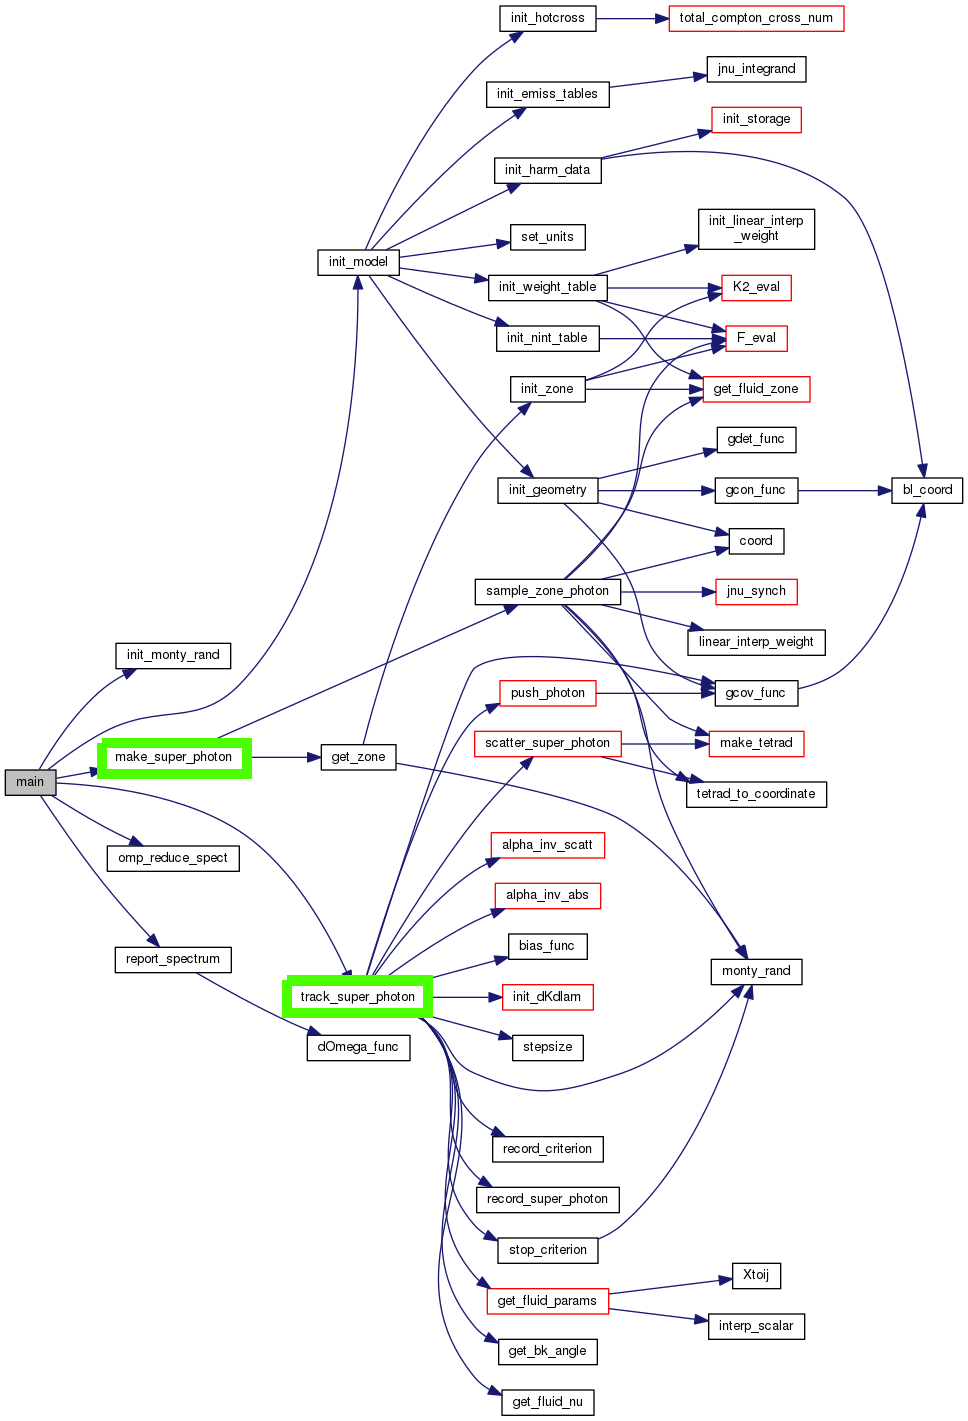
\includegraphics[width=.80\textwidth]{grmonty_graph.png}
    \caption{Grafo de chamadas de funções do grmonty, com enfâse em verde para a track e a make super photon}
    \label{fig:grmontyGraph}
  \end{figure}


  Dada a arquitetura do projeto, o foco principal para aumentar a performance é tornar a paralelização feita em OpenMP para CUDA. Para isso se faz necessário que todo o código previamente distribuido pelas threads do OpenMP tornem-se Kernels, funções device, funções que executam exclusivamente na GPGPU. As principais funções do grmonty que são feitas sob o OpenMP são a \textit{make\_super\_photon} e a \textit{track\_super\_photon} que possuem as responsabilidades de gerar um photon e rastrear a sua trajetória até o final, uma delas é também a função que demanda mais processamento. Para um N razoável capaz de gerar dados consistentes e interessantes 96,95\% do tempo de execução é na função \textit{track\_super\_photon} e sendo executada na ordem de cetenas de milhares de vezes, tornando essa função a mais interesante para ser massivamente paralelizada.

\section{Melhorias e Modificações}
  \subsection{OpenMP e Concorrência}
    O grmonty foi originalmente desenvolvido com OpenMP para maximar a paralelização, fazendo com que cada chamada a \textit{make\_super\_photon} e \textit{track\_super\_photon} fosse executada em paralelo e cada dupla de chamadas as duas funções rodaria em cada thread, isto só é possível porque cada fóton pode ser processado de maneira independente. Cada thread que cria e depois traça a trajetória das partículas é independente, porém ainda usam e consultam variáveis globais definidas no modelo criado na inicialização.

    Entretanto o processamento de cada thread, de cada fóton, pode ou não resultar na coleta final de um mais um fóton, para a verificar o ponto de parada do algorítmo se faz necessário que cada thread ao terminar, informe se obteve sucesso ou não e se obteve persistir os dados de seus resultados para análise posterior. Assim existe um ponto no código onde todas as threads tem que parar e esperar, enquanto uma delas acrescenta o valor total de partículas coletadas e armazena os seus dados. Esta tarefa é relativamente simples em OpenMP, como o código a baixo demonstra. Dois sinalizadores para o compilador fazem com que um treço de código rode como em uma região crítica, uma região onde somente uma thread pode entrar por vez:

    \begin{lstlisting}
void record_super_photon(struct of_photon *ph)
{
  /* inicializacao e verificacoes */
  /* codigo codigo codigo...      */

#pragma omp critical (MAXTAU)
  {
    /* max_tau_scatt eh variavel global externa*/
    if (ph->tau_scatt > max_tau_scatt)
      max_tau_scatt = ph->tau_scatt;
  }

  /* define em qual posicao salvar os dados */
  /* codigo codigo codigo codigo codigo...  */

#pragma omp atomic
  N_superph_recorded++; /* incrementa o numero fotons coletados */
#pragma omp atomic
  N_scatt += ph->nscatt;

  /* salva os dados */
  /* codigo...      */
}
    \end{lstlisting}

    É possível observar no código acima as directivas do OpenMP, as quais são responsáveis por assegurar que o código definido sob elas irá ser executado por apenas uma thread por vez, nunca duas ao mesmo tempo. Nota-se também que são usadas duas directivas diferentes, a \textit{\#pragma omp atomic} e a \textit{\#pragma omp critical (<TAG>) } (onde <TAG> pode ser um nome qualquer), Essas directivas tem uma função muito especial e difícil de ser reproduzida em CUDA.

    A biblioteca OpenMP possui algumas directivas especificas que informam o compilador certas regras ao gerar código, as duas vistas a cima tem essa função. A \textit{\#pragma omp atomic} é a mais simples, ela tem o objetivo de infomar o compilador que o trecho de código logo a baixo dela deve ser tratado como algo atômico, em outras palavras, que deve ser feito de uma única vez, não sendo permitido uma troca de contexto enquanto uma thread está sob essa directiva. O outro pragma é um pouco mais complexo, é o \textit{\#pragma omp critical (<TAG>) }, é possível  dizer que funciona como o anterior porém com algumas diferença. A primeira é a TAG, essa etiqueta é um nome qualquer escolhido pelo programador para identificar aquela região crítica de outras existentes no código. Enquanto o \textit{omp atomic} para toda e qualquer thread de atuar, o \textit{omp critical} somente vai impedir que outras threads no mesmo bloco identificado executem, isso lhe tras duas vantagens que a outra directiva não tem: códigos mais complexos podem ser executados, algo que não é permitido no \textit{omp atomic}, e o código lá executado não necessariamente vai bloquear toda a aplicação.

    Essas directivas do OpenMP funcionam por que são baseadas na POSIX threads api (POSIX), uma interface onde podem ser feitas chamadas ao sistema operacional e programas vão ser executados respeitando o padrão POSIX prestabelecido. Assim, já é conhecida e a muito tempo divulgada a interface com o CPU no que diz respeito programação multithread, porém no universo das GPGPUs esses padões não existem ou são muito novos.

    Em CUDA a duas directivas que o OpenMP faz podem ser implementadas, mas com uma dificuldade a mais. O \textit{\#pragma omp atomic} quanto utilizado para a soma, como no código a cima na linha 16 e 17 pode ser feito com a função CUDA \textit{atomicAdd} onde é possivel realizar uma soma em uma thread de forma atômica, sem que ocorra alguma condição de corrida entre as threads sendo possível atualizar o valor sem grandes problemas.

    A implementação já se complica quando tentamos trascrever a parte do código da região crítica. O bloco em questão é o das linhas 6 a 11, nele existem duas ações de resolução complicada, o condicional e a atribuição.

    A atribuição infelizmente não poderia ser implementada por um \textit{atomicAdd} como nas linhas 16 e 17, pois mesmo não sendo uma soma poderiamos escrever como se fosse. O trecho:
    \begin{lstlisting}
      max_tau_scatt = ph->tau_scatt;
    \end{lstlisting}

    poderia ser reescrito como:

    \begin{lstlisting}
      max_tau_scatt += (- max_tau_scatt + ph->tau_scatt);
    \end{lstlisting}

    mas ainda assim não funcionaria pois o \textit{atomicAdd} só realiza uma adição de forma atômica e a segunda forma precisa de duas adições e as duas tem quer ser feitas de uma vez. Isso é devido ao fato que ao se calcular o que deve ser adiconado a \textit{max\_tau\_scatt} utiliza-se o próprio \textit{max\_tau\_scatt} assim, é possível que o seu valor seja alterado por alguma outra thread entre o cálculo do o que deve ser adicionado e finalmente ser adicionado.

    Este dado já suficiente para descartamos o \textit{atomicAdd}, porém implementar uma região crítica a esse nível na GPGPU não é uma tarefa trivial, e devemos implementar um condicional também. Existem formas de criar regiões criticas na GPGPUs, como por exemplo o \textit{atomicCAS} que realiza uma comparação e dependendo do resultado faz uma atribuição ou não, tudo isso de forma atômica.

    Mas as threads em uma GPGPU não são independetes como as threads da CPU. As threads das GPGPUs e GPUs são agrupadas em grupos de 32, normalmente chamados de \textit{warps}. Todas as threads em um mesmo warp executam as intruções em uma forma completamente \textit{lock-step}, isto é, cada step que uma thread anda todas as outras também andam ao mesmo tempo. Se uma preposição de controle como um condicional ou um laço resulta em alguma ou algumas das 32 threads divergirem do resto, as threads remanecentes vão ficar em espera, dormindo, até as outras terminarem (cuda-c-best-practices-guide).

    No caso de implementar a região crítica utilizando o \textit{atomicCAS} para criar um mutex, deixaria algumas threads passarem enquanto outras ficariam esperando o mutex por um tempo indeterminado, uma vez que não há nada que enforce uma justica fraca no escalonamento das threads da GPU, resultando num programa que nunca terminaria, entrando em deadlock.

    Uma forma de resolver esse problema é permitindo que cada thread salve em um vetor compartilhado o valor de seu \textit{ph->tau\_scatt}, depois disso somente uma thread é encarregada de achar o maior valor e atribuir esse valor a \textit{max\_tau\_scatt}. A implementação dessa resolução está a baixo:

    \begin{lstlisting}
void record_super_photon(struct of_photon *ph)
{
  /* inicializacao e verificacoes */
  /* codigo codigo codigo...      */

  my_max_tau[thread_uniq_id] = ph->tau_scatt

  __syncthreads();

  if( thread_uniq_id == 0 ) /* somente uma das threads executa esse bloco */
    for(size_t i = 0; i < max_threads; i++){
      if(max_tau_scatt < my_max_tau[i])
        max_tau_scatt = my_max_tau[i]

  __syncthreads();

  /* define em qual posicao salvar os dados */
  /* codigo codigo codigo codigo codigo...  */

  atomicAdd(&N_superph_recorded, 1);
  atomicAdd(&N_scatt, ph->nscatt);

  /* salva os dados */
  /* codigo...      */
}
    \end{lstlisting}

    A biblioteca OpenMP trouxe grande potência e simplicidade para o código do grmonty, mas ao se utilizar a programação em GPGPUs como CUDA, usar em conjunto essa biblioteca pode não ser somente mais complcado como prejudicial a aplicação.

    Diferentemente da possibilidade de sempre ser possível criar um processo novo e lança-lo a CPU, isso nem sempre é possível na GPU, na realidade o lançamento de diversos kernels a GPGPU sem que ela tenah terminado um antes de vir o outro, pode tornar todo o processamento mais lento ou matar a aplicação que estava sendo executada anteriormente. Por motivos como esses não é uma boa prática tentar lançar vários kernel atraves do OpenMP.

    Como o OpenMP é amplamente usado no grmonty, porém somente em algumas áreas específicas seria interessante usar a programaçao em GPGPU, o código OpenMP continua presente em algumas partes da aplicação. Os trecho de código mais computacionalmente pesados e com potêncial para a a paralelização nestes sim é retirada a integração com o OpenMP e o código é portado para CUDA.

    Analisando o gráfico de processamento com indicação de performance, a figura \ref{fig:grmonty-performance} é evidente que o gargalo da aplicação é a função \textit{track\_super\_photon}. Por é que ela foi a escolhida para ser portada para a GPGPU, além de poder ser altamante paralelizável.

    \begin{figure}[!h]
      \centering
      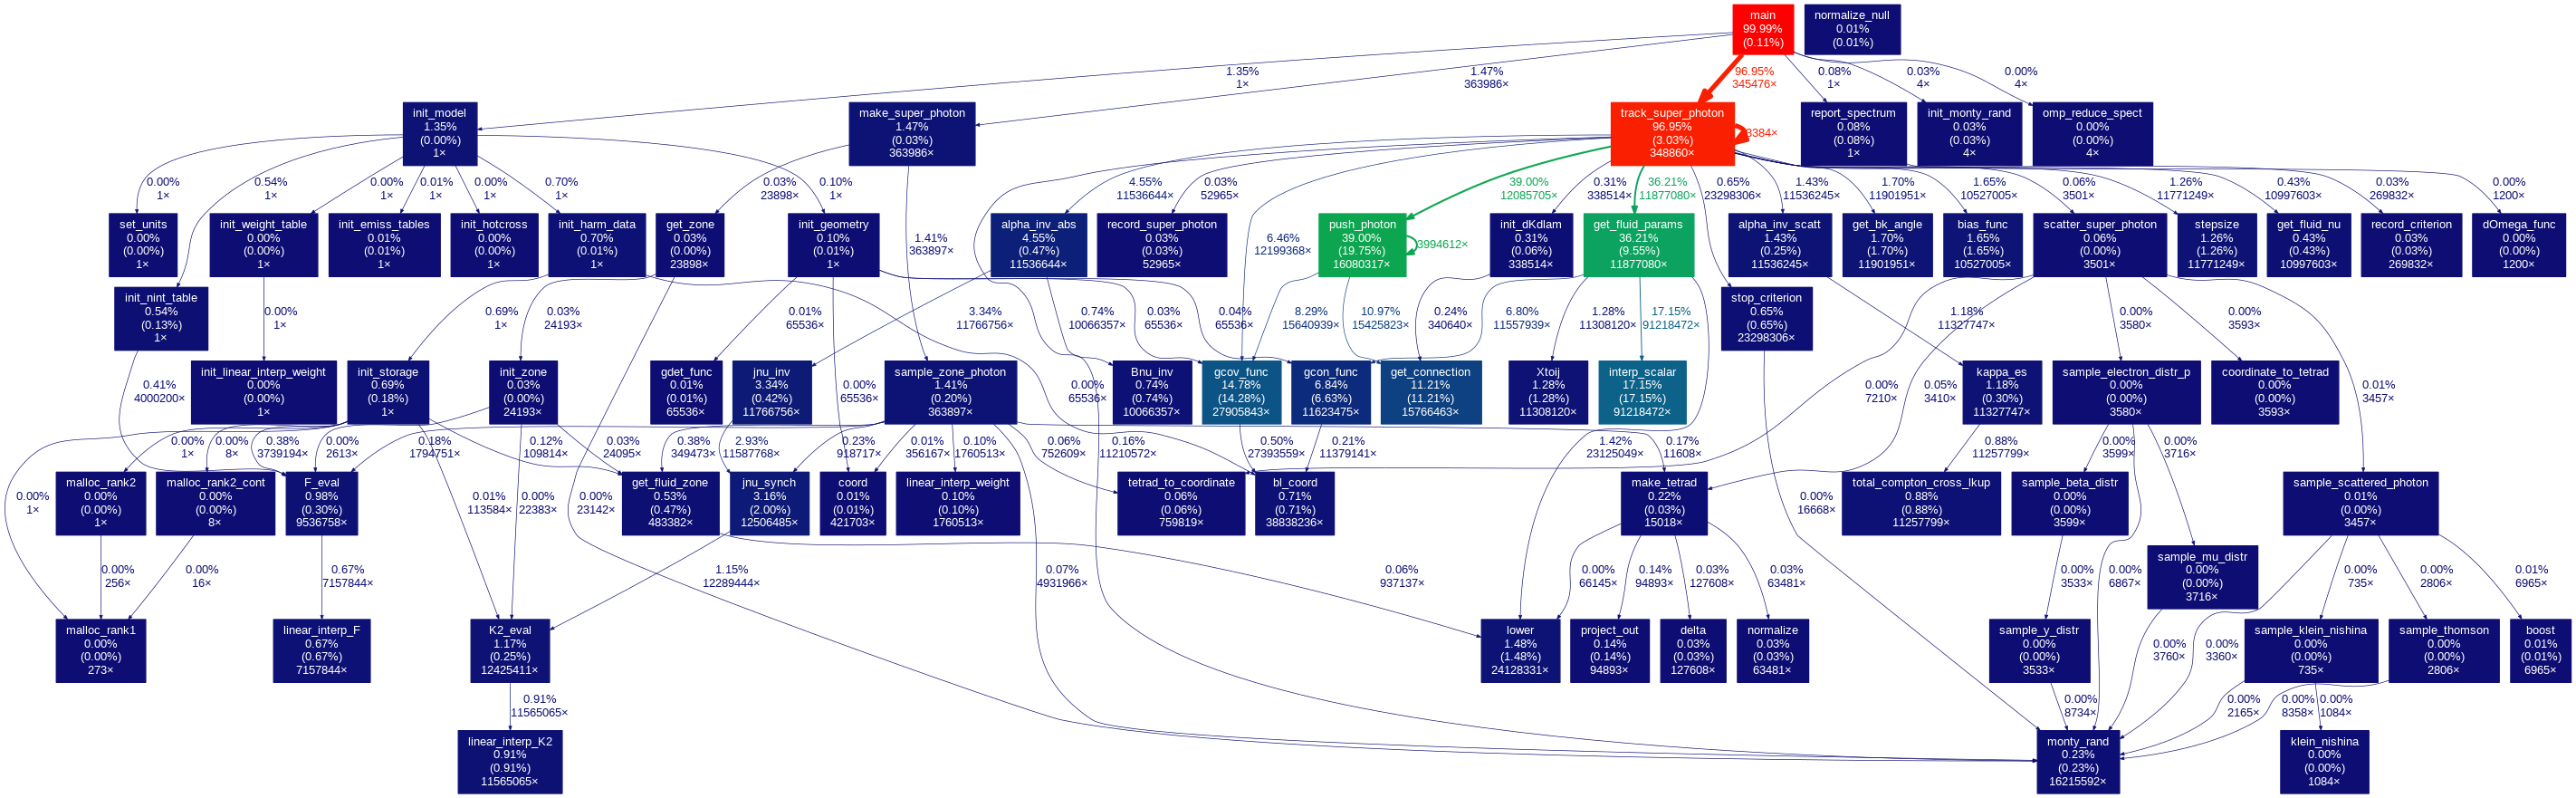
\includegraphics[width=.80\textwidth]{time_per_func.png}
      \caption{grafo de funcionamento do grmonty. Quanto mais vermelho mais tempo foi gasto. executados em um Ubuntu 17.10, x64, AMD Fx-6100 six-core processor, 8gb de ram. porcentagem tempo gasto até o retorno da função, porcentagem em parentesis é o tempo gasto somente dentro da função, não contando outras chamadas.}
      \label{fig:grmonty-performance}
    \end{figure}

  \subsection{math.h}
    Algumas funções matemáticas que o grmonty usa e que são implementadas pela gnu sentific library não poderem ser executadas na gpu uma vez que a não existe suporte para essas biblioteca pela a Nvidia, porém existe uma biblioteca similar da própria nvidia, a CUDAmath que aprensenta uma grande coleção de funções matemáticas que serviram como substitutas para as da gnu.

    O grmonty utiliza as funções:
    \begin{itemize}
      \item \textit{int gsl\_sf\_bessel\_Kn\_e(int n, double x, gsl_sf_result * result)} método de calcula a função de Bessel cilindrica modificada irregular de ordem n no ponto x
      \item \textit{void gsl\_ran\_dir\_3d(const gsl_rng * r, double * x, double * y, double * z)} Função que retorna
    \end{itemize}

    2 3 destas 1 e2 tem uma função identica  em sua bibliotexca, porem ela não possui essa função e para isso tivemos que codifica-la nos mesmos

    a funlçao emq eustao trata da criação de vetorner de tres dimensões e de ordem 1 aleátorios com uma dispeção uniforme.

    unix math pra nvida math
    quais funções
      qual funcionou
      qual não

  \subsection{divisão e trabalho e parelelização}
    o grmonty paralelizou sua carga de trabalho via OpenMP, desta forma o programa tem total acesso a memoria RAM e aos úcleos do processador. Todo o escalonamento de memória e processamneto é adminstrado pelo sistema operacional. A partir do momento que o código passa aser executado na GPGPU esse controle fino não tem como ser mais terceirizado a outro sistema, é de responsabilidade do programador administrar a memória e threads na GPGPU.

    A GPGPU utilizada nos testes é uma Nvida Geforce GTX 550TI, com 192 núcleos e 1024 Mb de memória. Para utilizar o máximo desse aparelho é necessário mnadar cagars de trabalho que utilizem todos os recursos na capacidade mais próxima a da máxima. Ao se utilizar, por exemplo um acarga de tralho de 1100 Mb um primeiro passo de execução usaria 100\% da memória porém o próximo usaria cerca de 10\% da memóra disponível, tonando 90\% da memória inativa. A mesma lógica pode ser aplica a GPGPU, deve-se priorizar por dividir o numero de threads que deseja que  kernel processe por um multiplo de 192, caso a diferença seja muito grande, garnde parte do núclos ficara inativa, dispendição recursos e tempo de alocação para o que não foi usado.

    Esa peculariedade da programaçãoe m gpus torna cada progtrama tendo a necessidade de se re configurara a cada computador novo ao qual se pretende executa-lo, porem é possivel programar a alocação de recusros para que sempre sdea a maior possivel.

    Existe uma api na tecnologia cuda que permite a bsuca por parametros dos dspositivos disponiveis para o processamento. com isso todo omrograma antes de lançar seus kernels pode buscar e configuar-se para otimizar o uso de resrsos. por exemplo, para o suso otimoização do núclos das GPGPU é feita tal conta pra distruir as thrads em blocos na grind de execução das threads

    enquanto a memoria se faz necesario medir o tamanhos da ststruturas necessárias e tambepm o possicvel espaço máximo que o progrma pode vier a ter que usar dorante a sua execução pis caso ultrapasse o que a GPUoferecxe o proma pode não coneguir rodar.



  \subsection{Processar em Lotes}
    Uma mudança muito importante que deve ser feitapara tornar possivel a aparalelização na gpu e tornama imais eficiente é  mudar o modo de operaçõ do grmonty. atualmete ele cria um fotoon para um rasteio, é uam relação um pra um onde ná ha persistenca, ou acumooulo de photons para dai serem processados.

    No modelo  de GPGPu uma mudanlça para a maior perfimance seria mudar esse modelo de processamneto permitindo que lele posa ocorrer em for ma de batch, isot é um con juto de photos é produxido e armazenadopara sobemente no memomento ue chegasse ao tamanho otimo para ser executado na gpgpu ele fio kerern fosse lançado,

    para essa modificação é ncessario armazer uma uamg rnad quantode de fontos iniciando  make duper foton diversas vezxes ate se conseguir um tamanho toimo de ocupação na gou e que tambem nao fazço o prcessamento no ser eficinetre na gpgpgu isso é qeu qque nçao haja nucluo=s ociosos no processamento ou melhor que haja o menor numeotr possiveis deles.

    de ``assim que possível'' ``para processamento em lotes''
